\documentclass[handout]{beamer}
\setbeameroption{hide notes}
%show notes on second screen=right
%show only notes
%hide notes
%[handout]

\usepackage{esint}
\usepackage{graphicx}
\usepackage{tikz}
\usepackage{caption}
\usepackage{subcaption}
\usepackage[british]{babel}
\usepackage{mathtools}
\usepackage{appendixnumberbeamer}

\usepackage{csquotes}
\usepackage[style=verbose,backend=biber]{biblatex}
\bibliography{beamer}
%\usepackage{kpfonts}

% Theme (Boadilla, Hannover, metropolis, Pittsburgh)

% METROPOLIS
% Uses Fira fonts - compile with xelatex to use
% Features [standout] frames

%background=dark/light
\usetheme[progressbar=frametitle, background=dark]{metropolis}
\setbeamercolor{normal text}{fg=white}

% Colours (owl, dolphin, seagull)

% OWL
% Custom colours: red, green, blue, cyan, brown, orange, yellow, violet
% Has [snowy] variant

\usecolortheme{}
%\usebackgroundtemplate{\tikz\node[opacity=0.3]{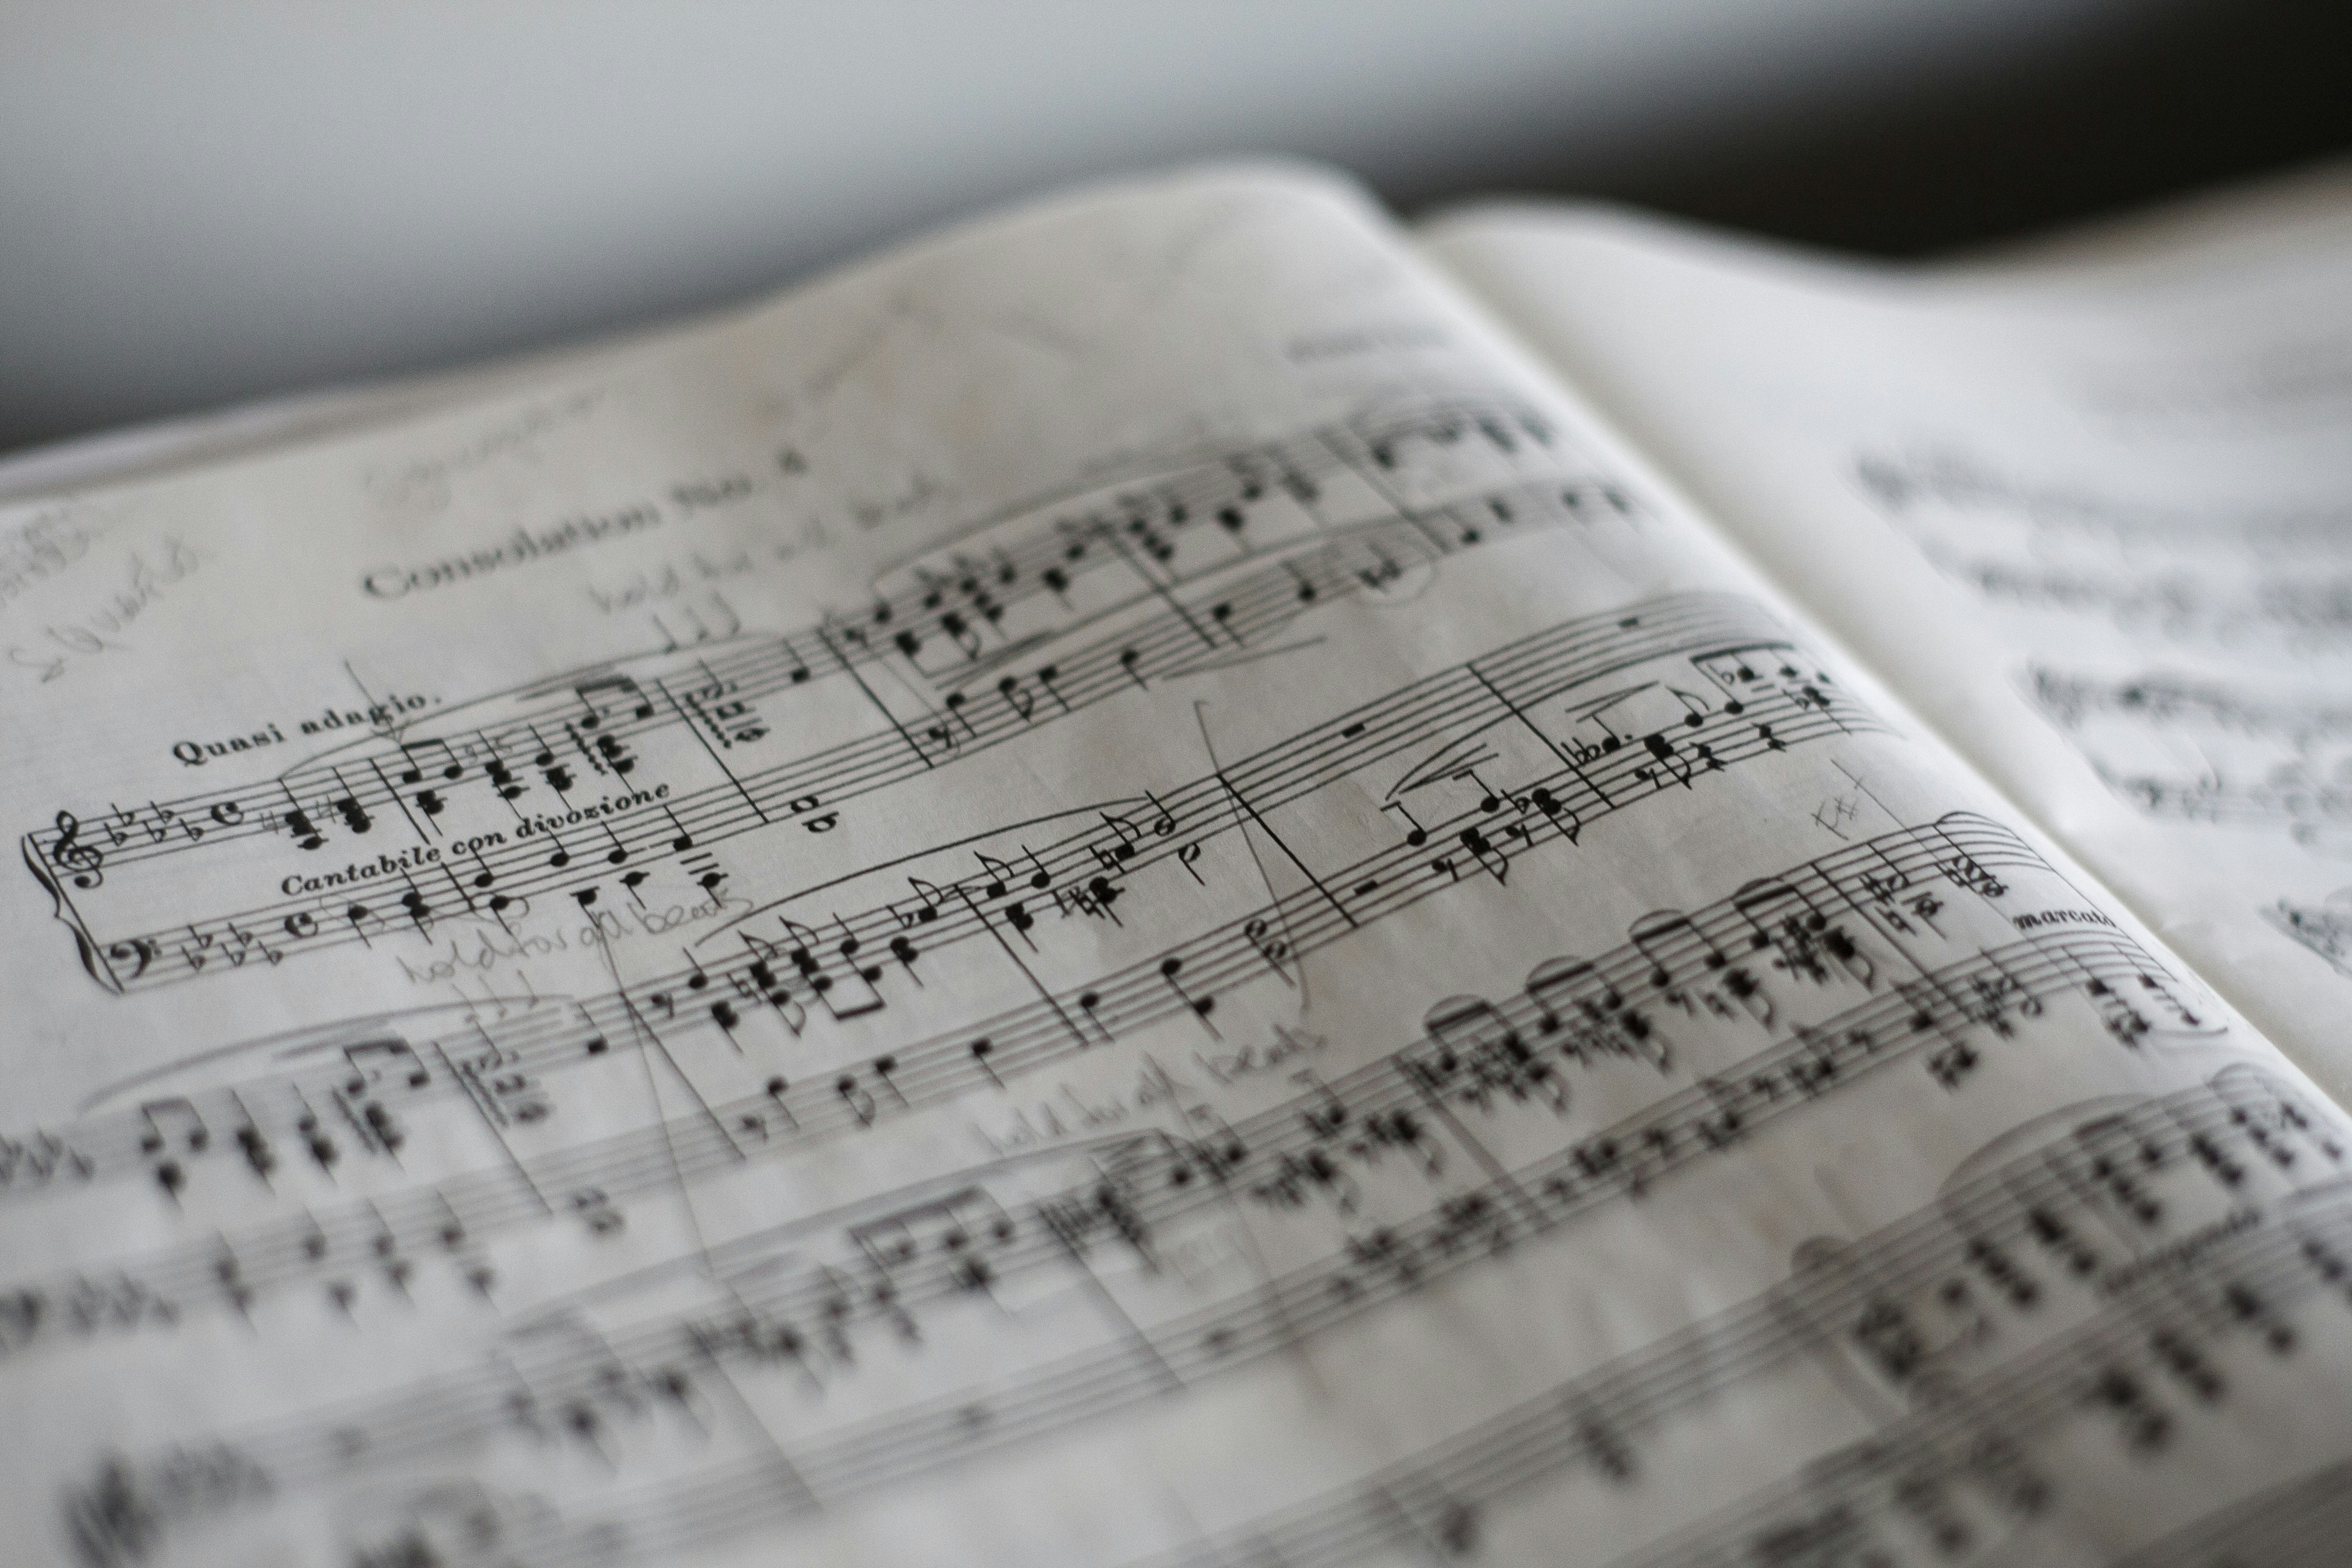
\includegraphics[width=\paperwidth,height=\paperheight]{../Figures/manuscript.jpg}};}

\setbeamerfont{caption}{size=\tiny}         % Caption size
\captionsetup[figure]{labelformat=empty}    % Remove figure labels
\captionsetup[subfigure]{labelformat=empty}
\usefonttheme[onlymath]{serif}

%\logo{\includegraphics[height=2cm]{}}
\title{Quantum Annealing for Music Arrangement}
\author{Lucas Kirby}
\institute{Department of Physics, Durham University}
\date{4 March 2025}

\begin{document}

\begin{frame}
    \titlepage
\end{frame}

\begin{frame}{Overview}
    \tableofcontents

    \note<1->{\begin{itemize}
        \item{What is music arrangement? What is quantum annealing?}
        \item{Methods used to solve the music arrangement problem}
        \item{Preliminary results from application of the method}
        \item{Concluding thoughts about this process}
    \end{itemize}}
\end{frame}

\section{Motivations}

\begin{frame}{Motivations}
    
    \begin{itemize}
        \item Small lit review\footnotemark
        \item Quantum computer music
        \item My own novel adaption of the method
        \item THIS IS MY OWN IDEA
    \end{itemize}
    
    \tiny\footnotetext{\tiny\cite{cambouropoulos_lbdm_2011}}
\end{frame}

\section{Theory} %%%%%%%%%%

\subsection{Music arrangement}

\begin{frame}{Music arrangement}
    \begin{columns}
        \begin{column}{0.6\textwidth}
            \begin{itemize}[<+(1)->]
                \item Adaptation of previously composed pieces for practical or artistic reasons
                \item Traditionally complex and time-consuming
                \item This study focuses on \textbf{reduction}
            \end{itemize}
        \end{column}
        \begin{column}{0.4\textwidth}
            \begin{figure}
                \centering
                    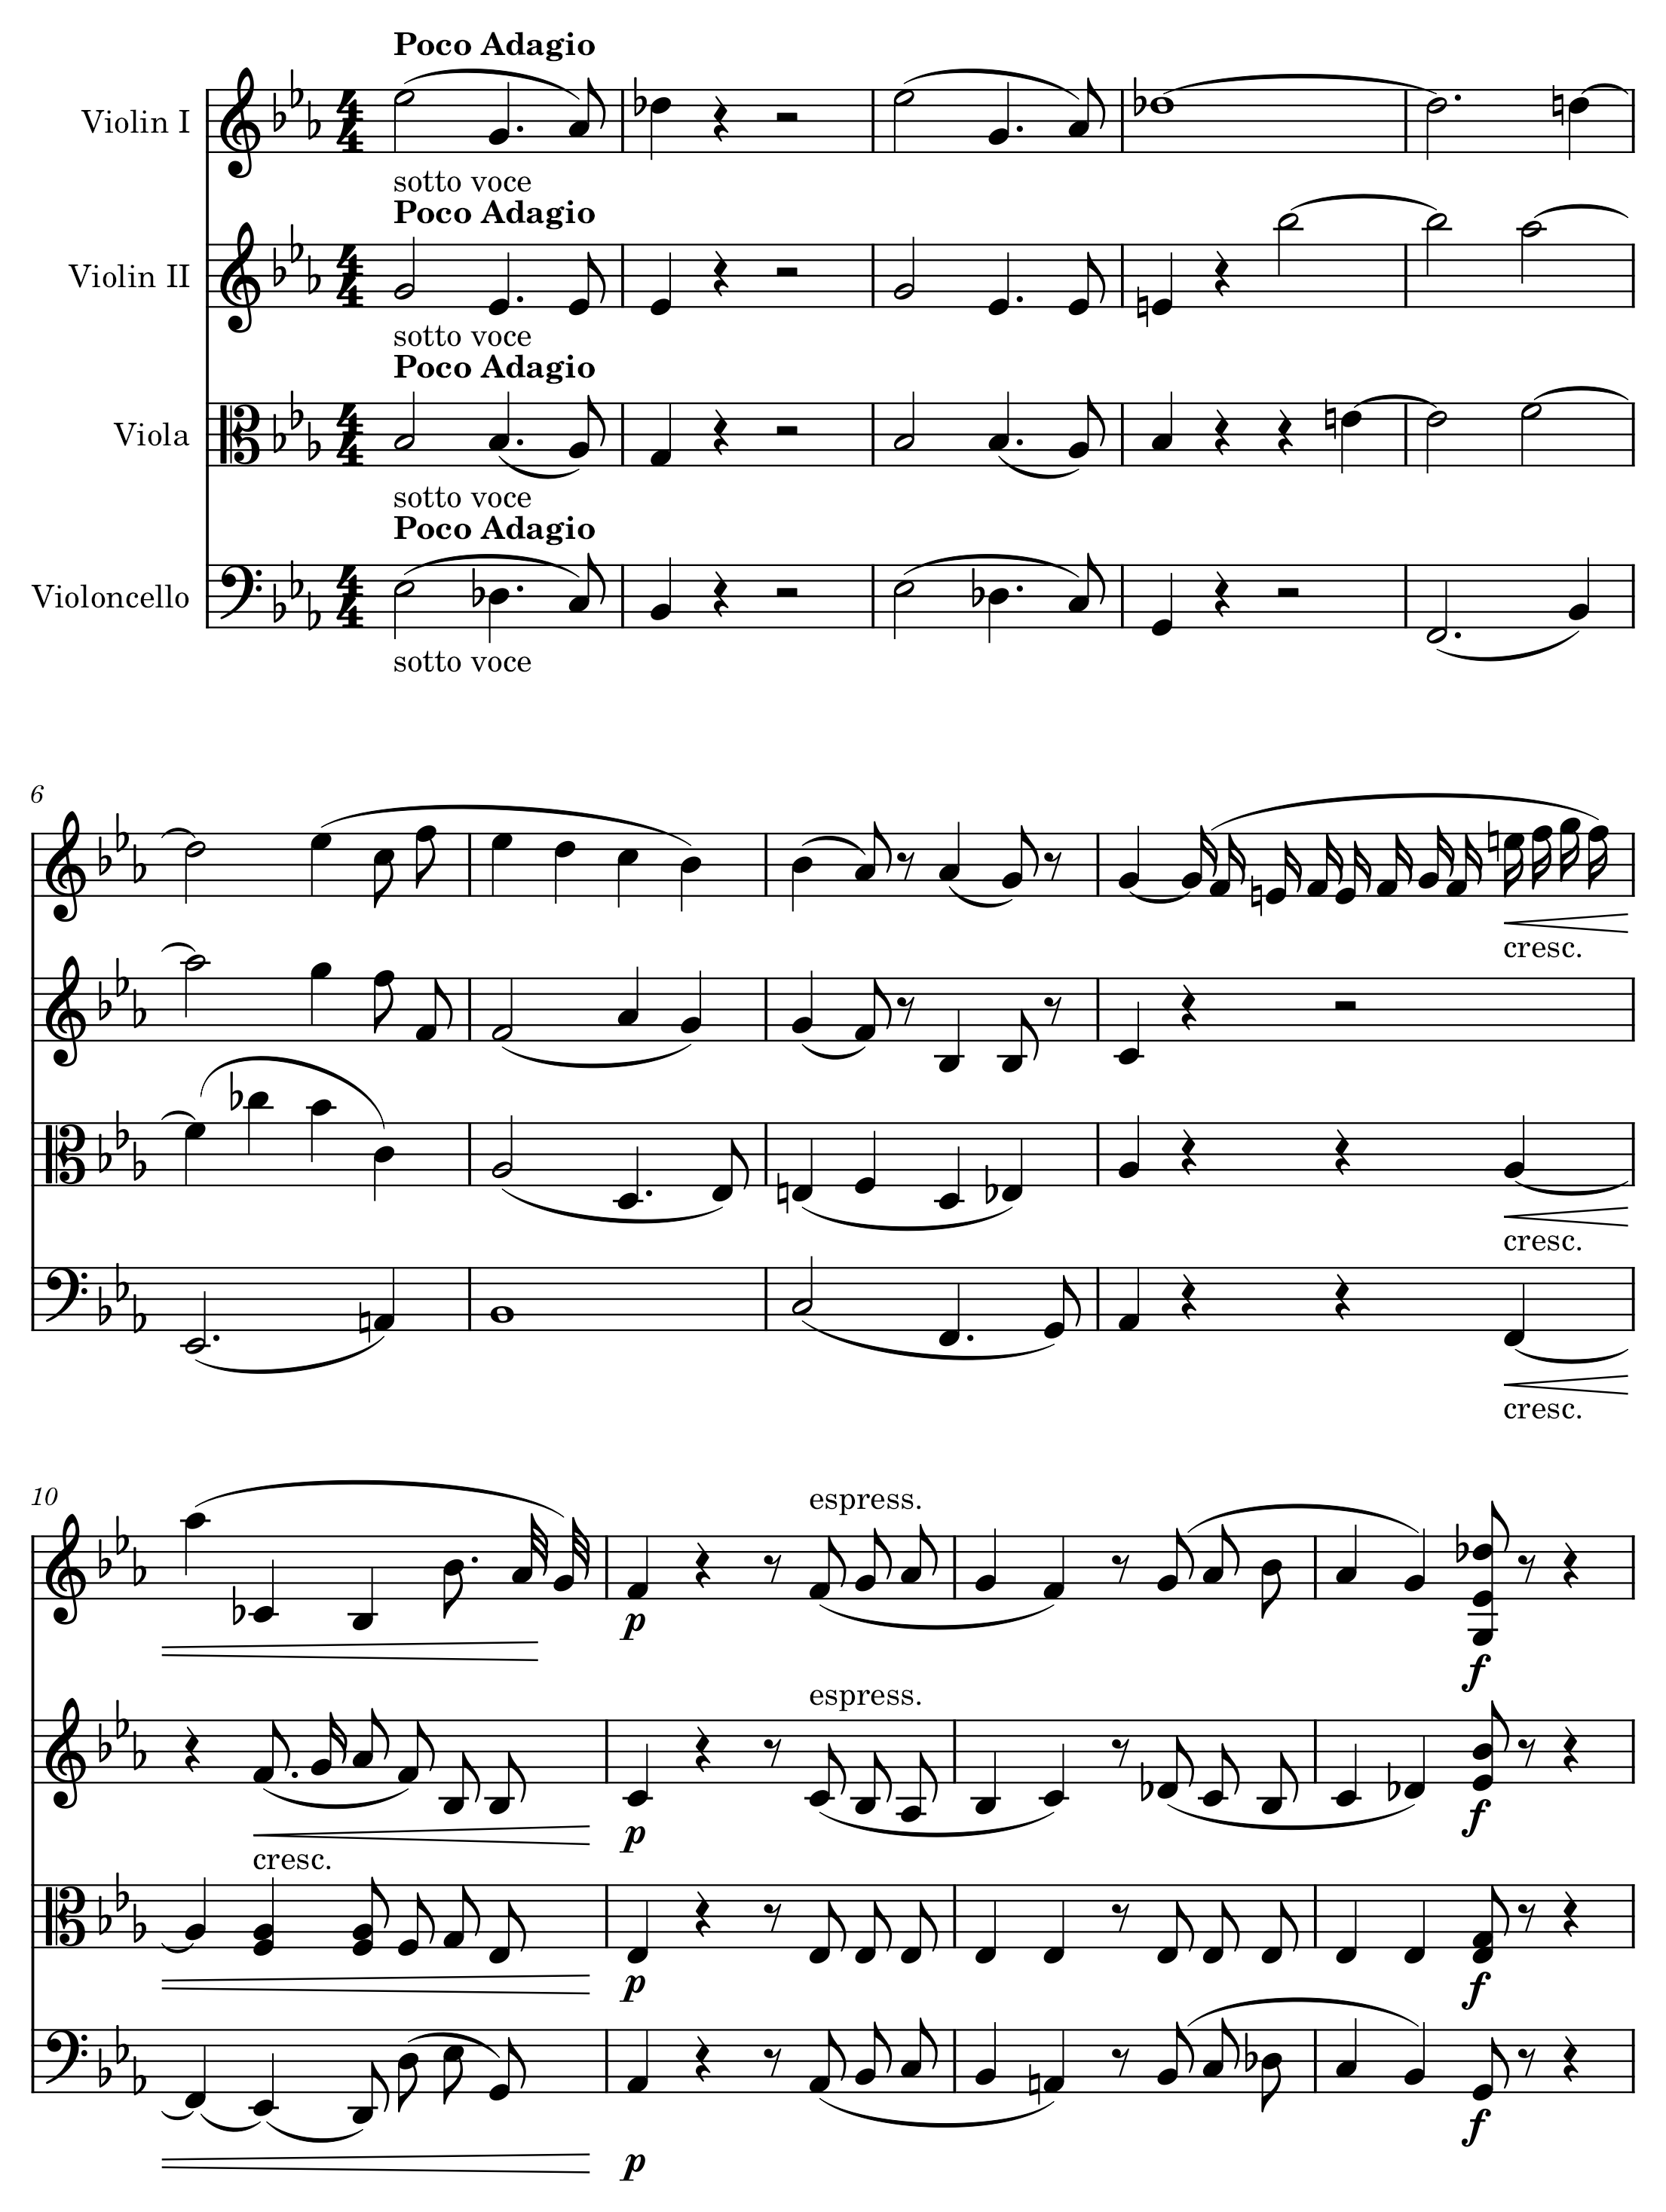
\includegraphics[width=\textwidth]{../Figures/excerpt-1.png}
                    \caption{Beethoven's String Quartet No.\ 10}
                \end{figure}
        \end{column}
    \end{columns}
    
    \note<1->{\begin{itemize}
        \item Adaptation of music in terms of instrumentation, medium, or style
        \item Traditionally a complex process that requires a deep understanding of musical theory and structure
        \item Musically interesting whilst still remaining faithful to the source material
        \item Interest in automating this process
        \item Reduction is the rewriting of music for a smaller number of instruments (for example string quartet)
    \end{itemize}}
\end{frame}


\subsection{Quantum annealing}

\begin{frame}{Adiabatic quantum computing (AQC)}
    \begin{itemize}[<+(1)->]
        \item \emph{Materials} | heating and cooling a material to alter its physical properties
        \item \emph{Quantum} | changing a quantum system from one Hamiltonian to another
        \item Done slowly and adiabatically to remain in the ground state
    \end{itemize}
    \pause
    \vfill
    \begin{equation*}
        H(t)=\left(1- \frac{t}{T}\right)H_0 + \frac{t}{T}H_p
    \end{equation*}
    \hfill\cite{lucas_ising_2014}
    
    \note<1->{\begin{itemize}
        \item Materials science, annealing is a slow heating/cooling process to make a material softer and less brittle
        \item Quantum computing, slow evolution of a system between Hamiltonians
        \item Done adiabatically (closed system), system remains in ground state
    \end{itemize}}
\end{frame}

\begin{frame}{Quantum annealing}
    \pause
    \begin{exampleblock}{Ising model}
        \begin{equation*}
            H_p(\sigma^z) = \sum^N_{i<j}J_{ij}\sigma^z_i \sigma^z_j + \sum_{i=1}^{N}h_i \sigma^z_i
        \end{equation*}
    \end{exampleblock}
    \pause
    \begin{alertblock}{Initial state}
        \begin{equation*}
            H_0 = h_0\sum_{i=1}^{N}\sigma_i^x
        \end{equation*}
    \end{alertblock}
    \hfill\cite{lucas_ising_2014}
    
    \note<1->{\begin{itemize}
        \item{How is this used to solve problems?}
        \item{Ising model, create a lattice of variables with two discrete values (spin up/down)}
        \item{Problem Hamiltonian, qubits $\sigma^z$, coupling strengths $J_{ij}$ and field strengths $h_i$}
        \item{Initial state is a superposition of all possible states}
        \item{If problem solution is encoded within the ground state, system will give solution after evolution}
    \end{itemize}}
\end{frame}

\begin{frame}{Quantum annealing}

    \note<1->{\begin{itemize}
        \item{What does this look like?}
        \item{Evolution of superposition to a particular state}
        \item{More efficiently escape from local minima via quantum tunneling}
        \item{Can solve harder problems with a more turbulent energy landscape}
    \end{itemize}}
\end{frame}

\begin{frame}{QUBO}
    \pause
    \begin{block}{Quadratic Unconstrained Binary Optimisation}
        \vspace{0.1em}
        \begin{equation*}
            f(x)=\alert<+(1)>{\sum^N_{i<j}Q_{i,j}x_ix_j} + \alert<+(1)>{\sum^N_iQ_{i,i}x_i}
        \end{equation*}
    \end{block}
    \pause
    \begin{itemize}
        \item Encodes problem solution into Hamiltonian's ground state
        \item Sent to the QPU for optimisation
    \end{itemize}

    \note<1->{\begin{itemize} 
        \item{How to encode a problem into a Hamiltonian?}
        \item{Similar form to the Ising model, but with binary variables (0 or 1)}
        \item{QUBO is a function to be minimised}
        \item{Set of binary variables $x$, matrix $Q$ of real weights that describes interactions between variables}
        \item{Can read out variable values after evolution to give solution}
    \end{itemize}}
\end{frame}

\begin{frame}[standout]
    How to combine them?

    \note<1->{\begin{itemize}
        \item{How to apply quantum annealing to the problem of music arrangement?}
    \end{itemize}}
\end{frame}

\section{Methods} %%%%%%%%%%

\begin{frame}{Problem formulation}
    \begin{enumerate}[<+(1)->]
        \item Split score into musical phrases
        \item Arrange phrases into a graph
        \item Solve graph problem using QPU
        \item Construct arrangement from solution
    \end{enumerate}

    \note<1->{\begin{itemize}
        \item{Formulating arrangement as a problem to be solved via annealing, four-step process}
        \item{Split parts into musical phrases}
        \item{Arrange phrases into a graph (nodes and edges)}
        \item{Solve corresponding graph problem using quantum computing}
        \item{Construct final arrangement from the solution returned}
    \end{itemize}}
\end{frame}

\begin{frame}{1.\ Split score}
    \pause
    \begin{block}{Local boundary detection model (LBDM)}
        \vspace{0.1em}
        \begin{equation*}
            S_i=x_i\times (r_{i-1, i} + r_{i, i+1})
        \end{equation*}
        \hfill \cite{cambouropoulos_lbdm_2011}
    \end{block}
    \pause
    \begin{figure}
        \includegraphics<1->[width=0.8\textwidth]{../Figures/toy-1.png}
    \end{figure}

    \note<1->{\begin{itemize}
        \item{First stage to separate each part of original score into phrases}
        \item{Phrases | smallest unit of music that preserves melody and structure}
        \item{Boundaries between phrases found using LBDM}
        \item{Measures the degree of change of a certain parameter between notes (explain equation)}
        \item{Check pitch and IOI}
        \item{Strengths above a threshold value are considered phrases}
    \end{itemize}}
\end{frame}

\begin{frame}{2.\ Create graph}
    \begin{figure}
        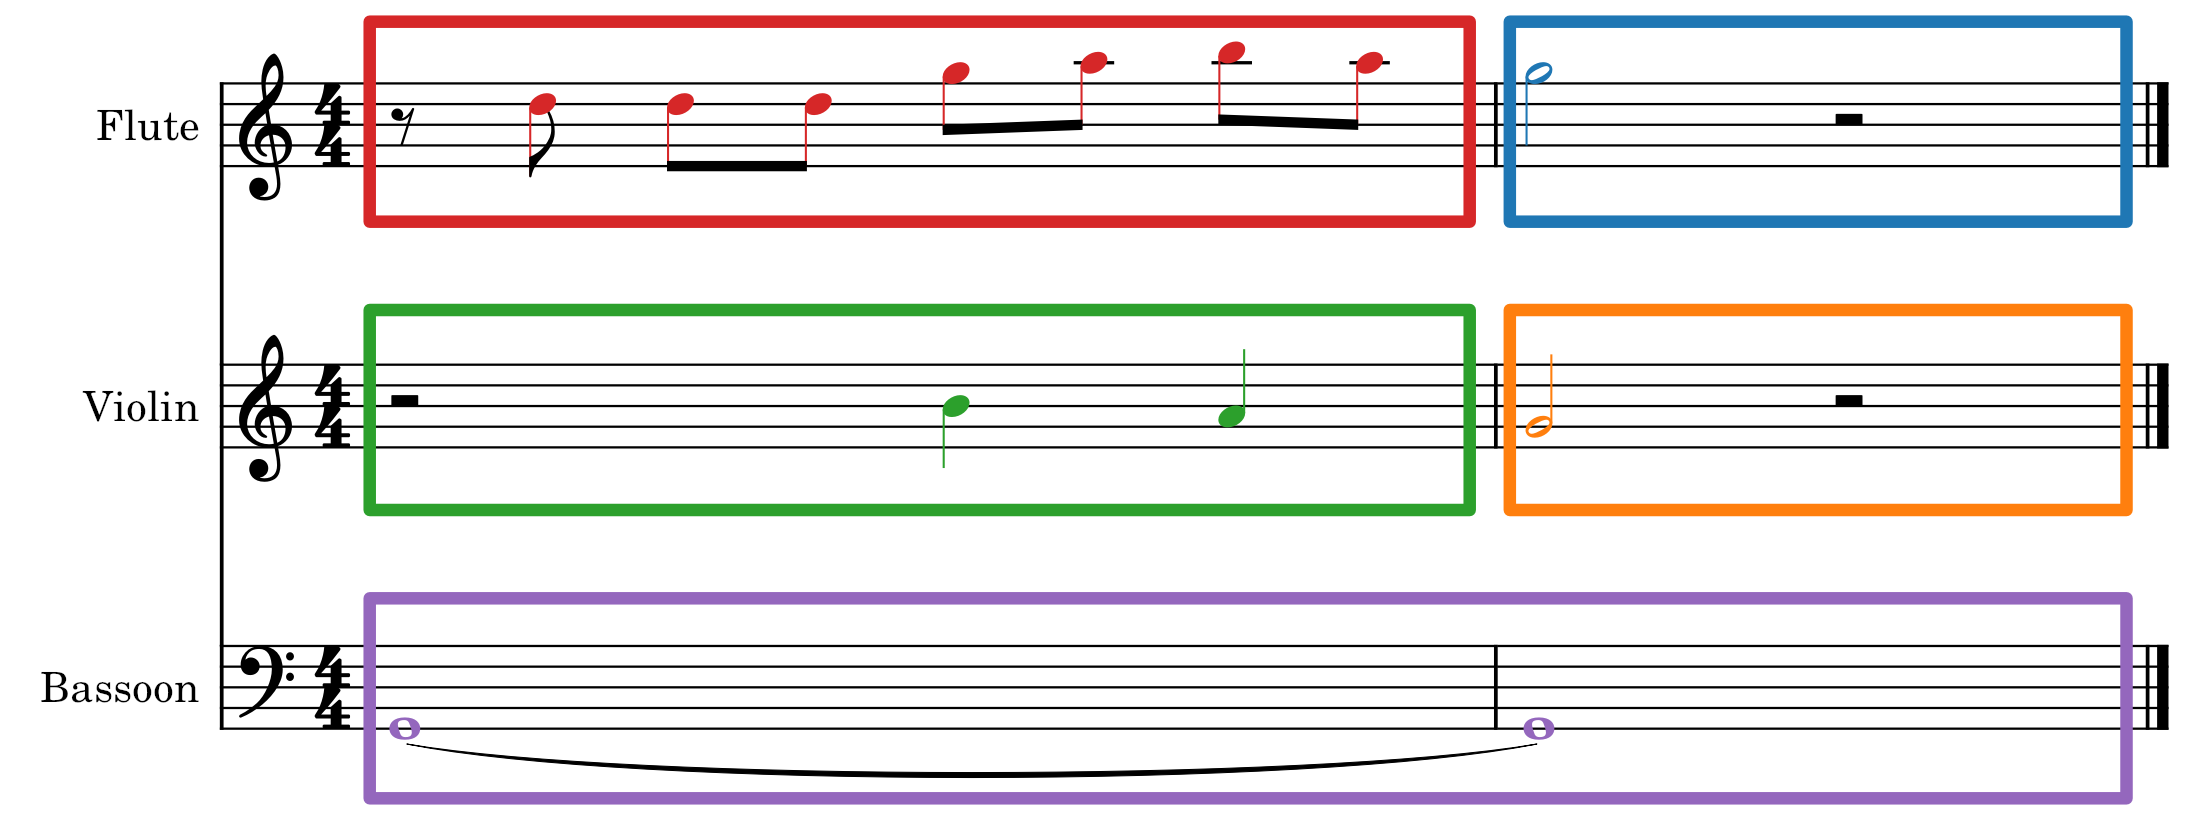
\includegraphics[width=0.8\textwidth]{../Figures/toy-1.png}
    \end{figure}
    \pause
    \begin{figure}
        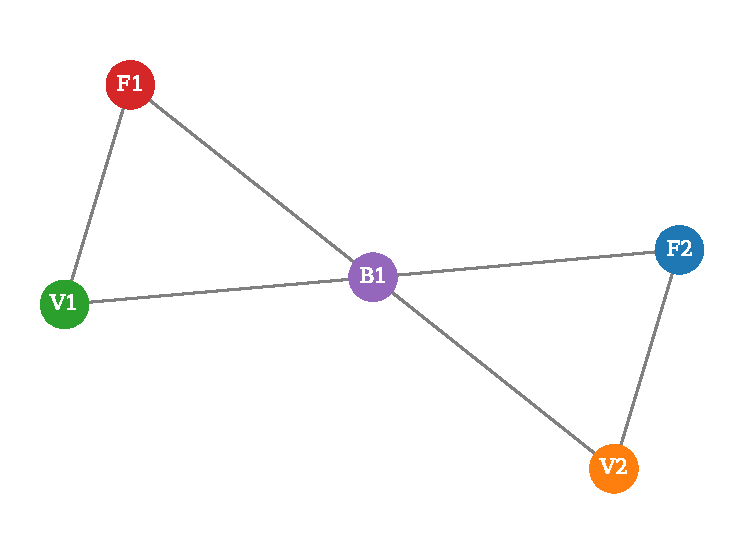
\includegraphics[width=0.5\textwidth]{../Figures/toy_graph.pdf}
    \end{figure}

    \note<1->{\begin{itemize}
        \item{Construct problem graph}
        \item{Each phrase becomes a node, edges between nodes if phrases overlap}
    \end{itemize}}
\end{frame}

\begin{frame}{3.\ Solve graph}
    \uncover<2->{\begin{alertblock}{Maximal independent set (MIS)}
        \vspace{0.1em}
        Largest subset of nodes such that no nodes within the subset are connected by an edge}
    \end{alertblock}
    \begin{columns}
        \begin{column}{0.5\textwidth}
            \begin{figure}
                \includegraphics<1->[width=0.9\textwidth]{../Figures/toy_graph.pdf}
            \end{figure}
        \end{column}
        \begin{column}{0.5\textwidth}
            \begin{figure}
                \includegraphics<3->[width=0.9\textwidth]{../Figures/toy_solution.pdf}
            \end{figure}
        \end{column}
    \end{columns}

    \note<1->{\begin{itemize}
        \item{Special case for reducing to a single monophonic part (one phrase played at a time)}
        \item{Solve problem graph using a graph theory problem called MIS}
        \item{Enforces that only one simultaneous phrase can be played at once}
        \item{Nodes can also be weighted to introduce preference for certain nodes e.g.\ musicality}
        
    \end{itemize}}
\end{frame}

\begin{frame}{4.\ Construct arrangement}
    \begin{figure}
        \begin{subfigure}{0.6\linewidth}
            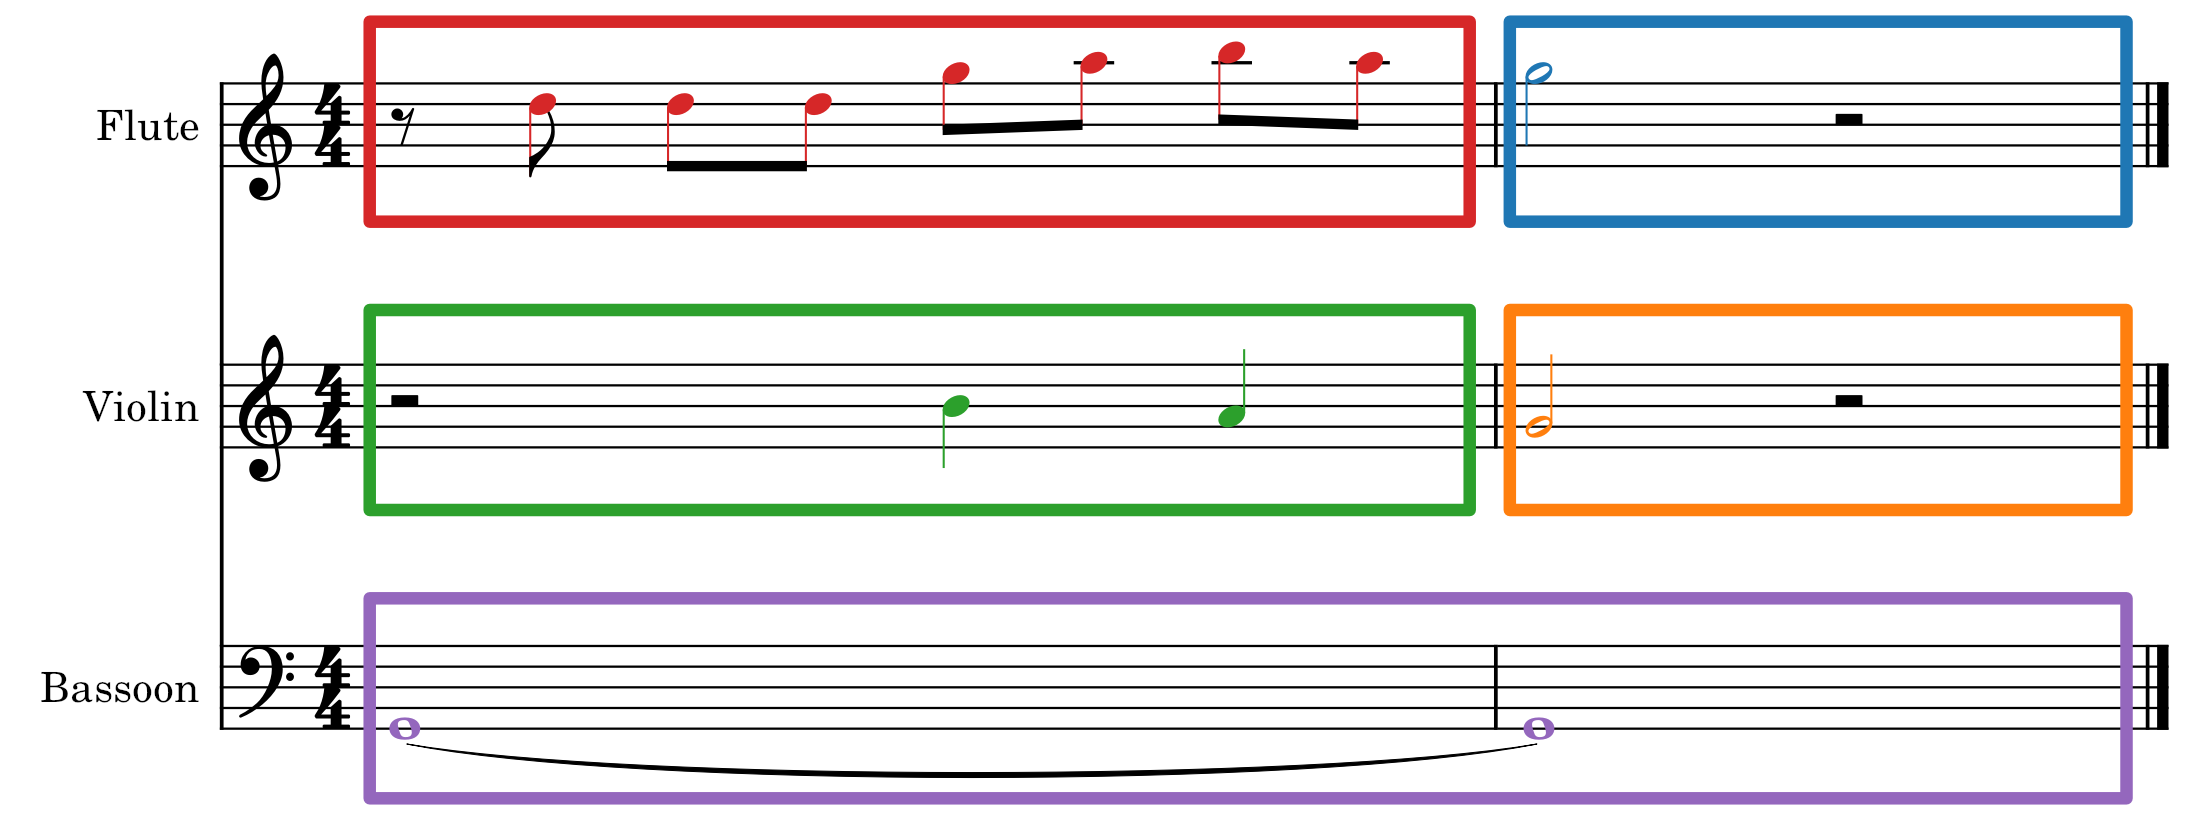
\includegraphics[width=0.9\linewidth]{../Figures/toy-1.png}
        \end{subfigure}\hfill
        \begin{subfigure}{0.4\linewidth}
            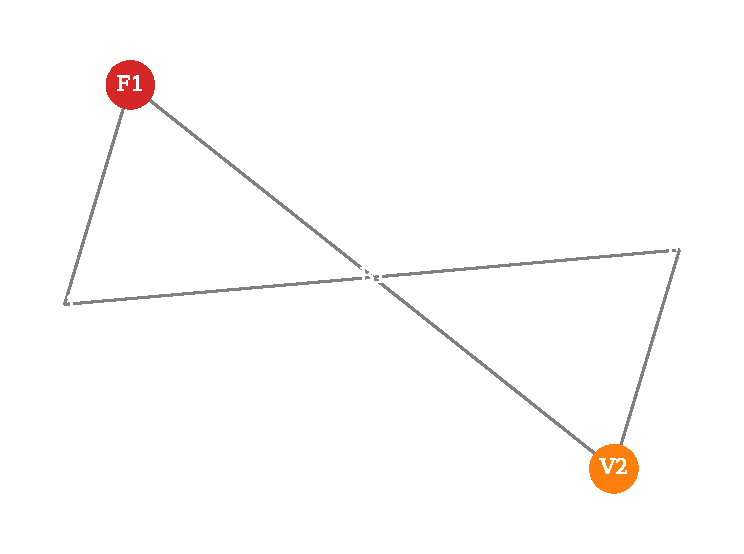
\includegraphics[width=0.9\linewidth]{../Figures/toy_solution.pdf}
        \end{subfigure}
    \end{figure}
    \pause
    \centering
    \begin{tikzpicture}
        \draw [thick, -latex](0,0) -- (0,-1);
    \end{tikzpicture}
    \begin{figure}
        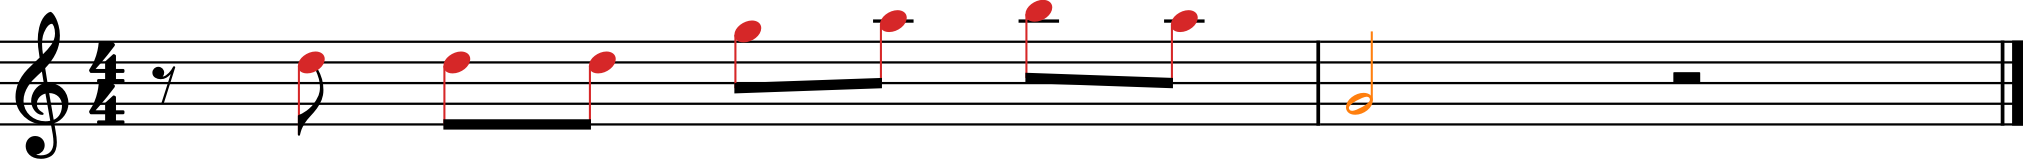
\includegraphics[width=0.8\textwidth]{../Figures/toy_arrangement-1.png}
    \end{figure}

    \note<1->{\begin{itemize}
        \item{Take solution graph and combine selected nodes to create final arrangement}
    \end{itemize}}
\end{frame}

\section{Results} %%%%%%%%%%

\begin{frame}{Excerpt}
    \begin{figure}
        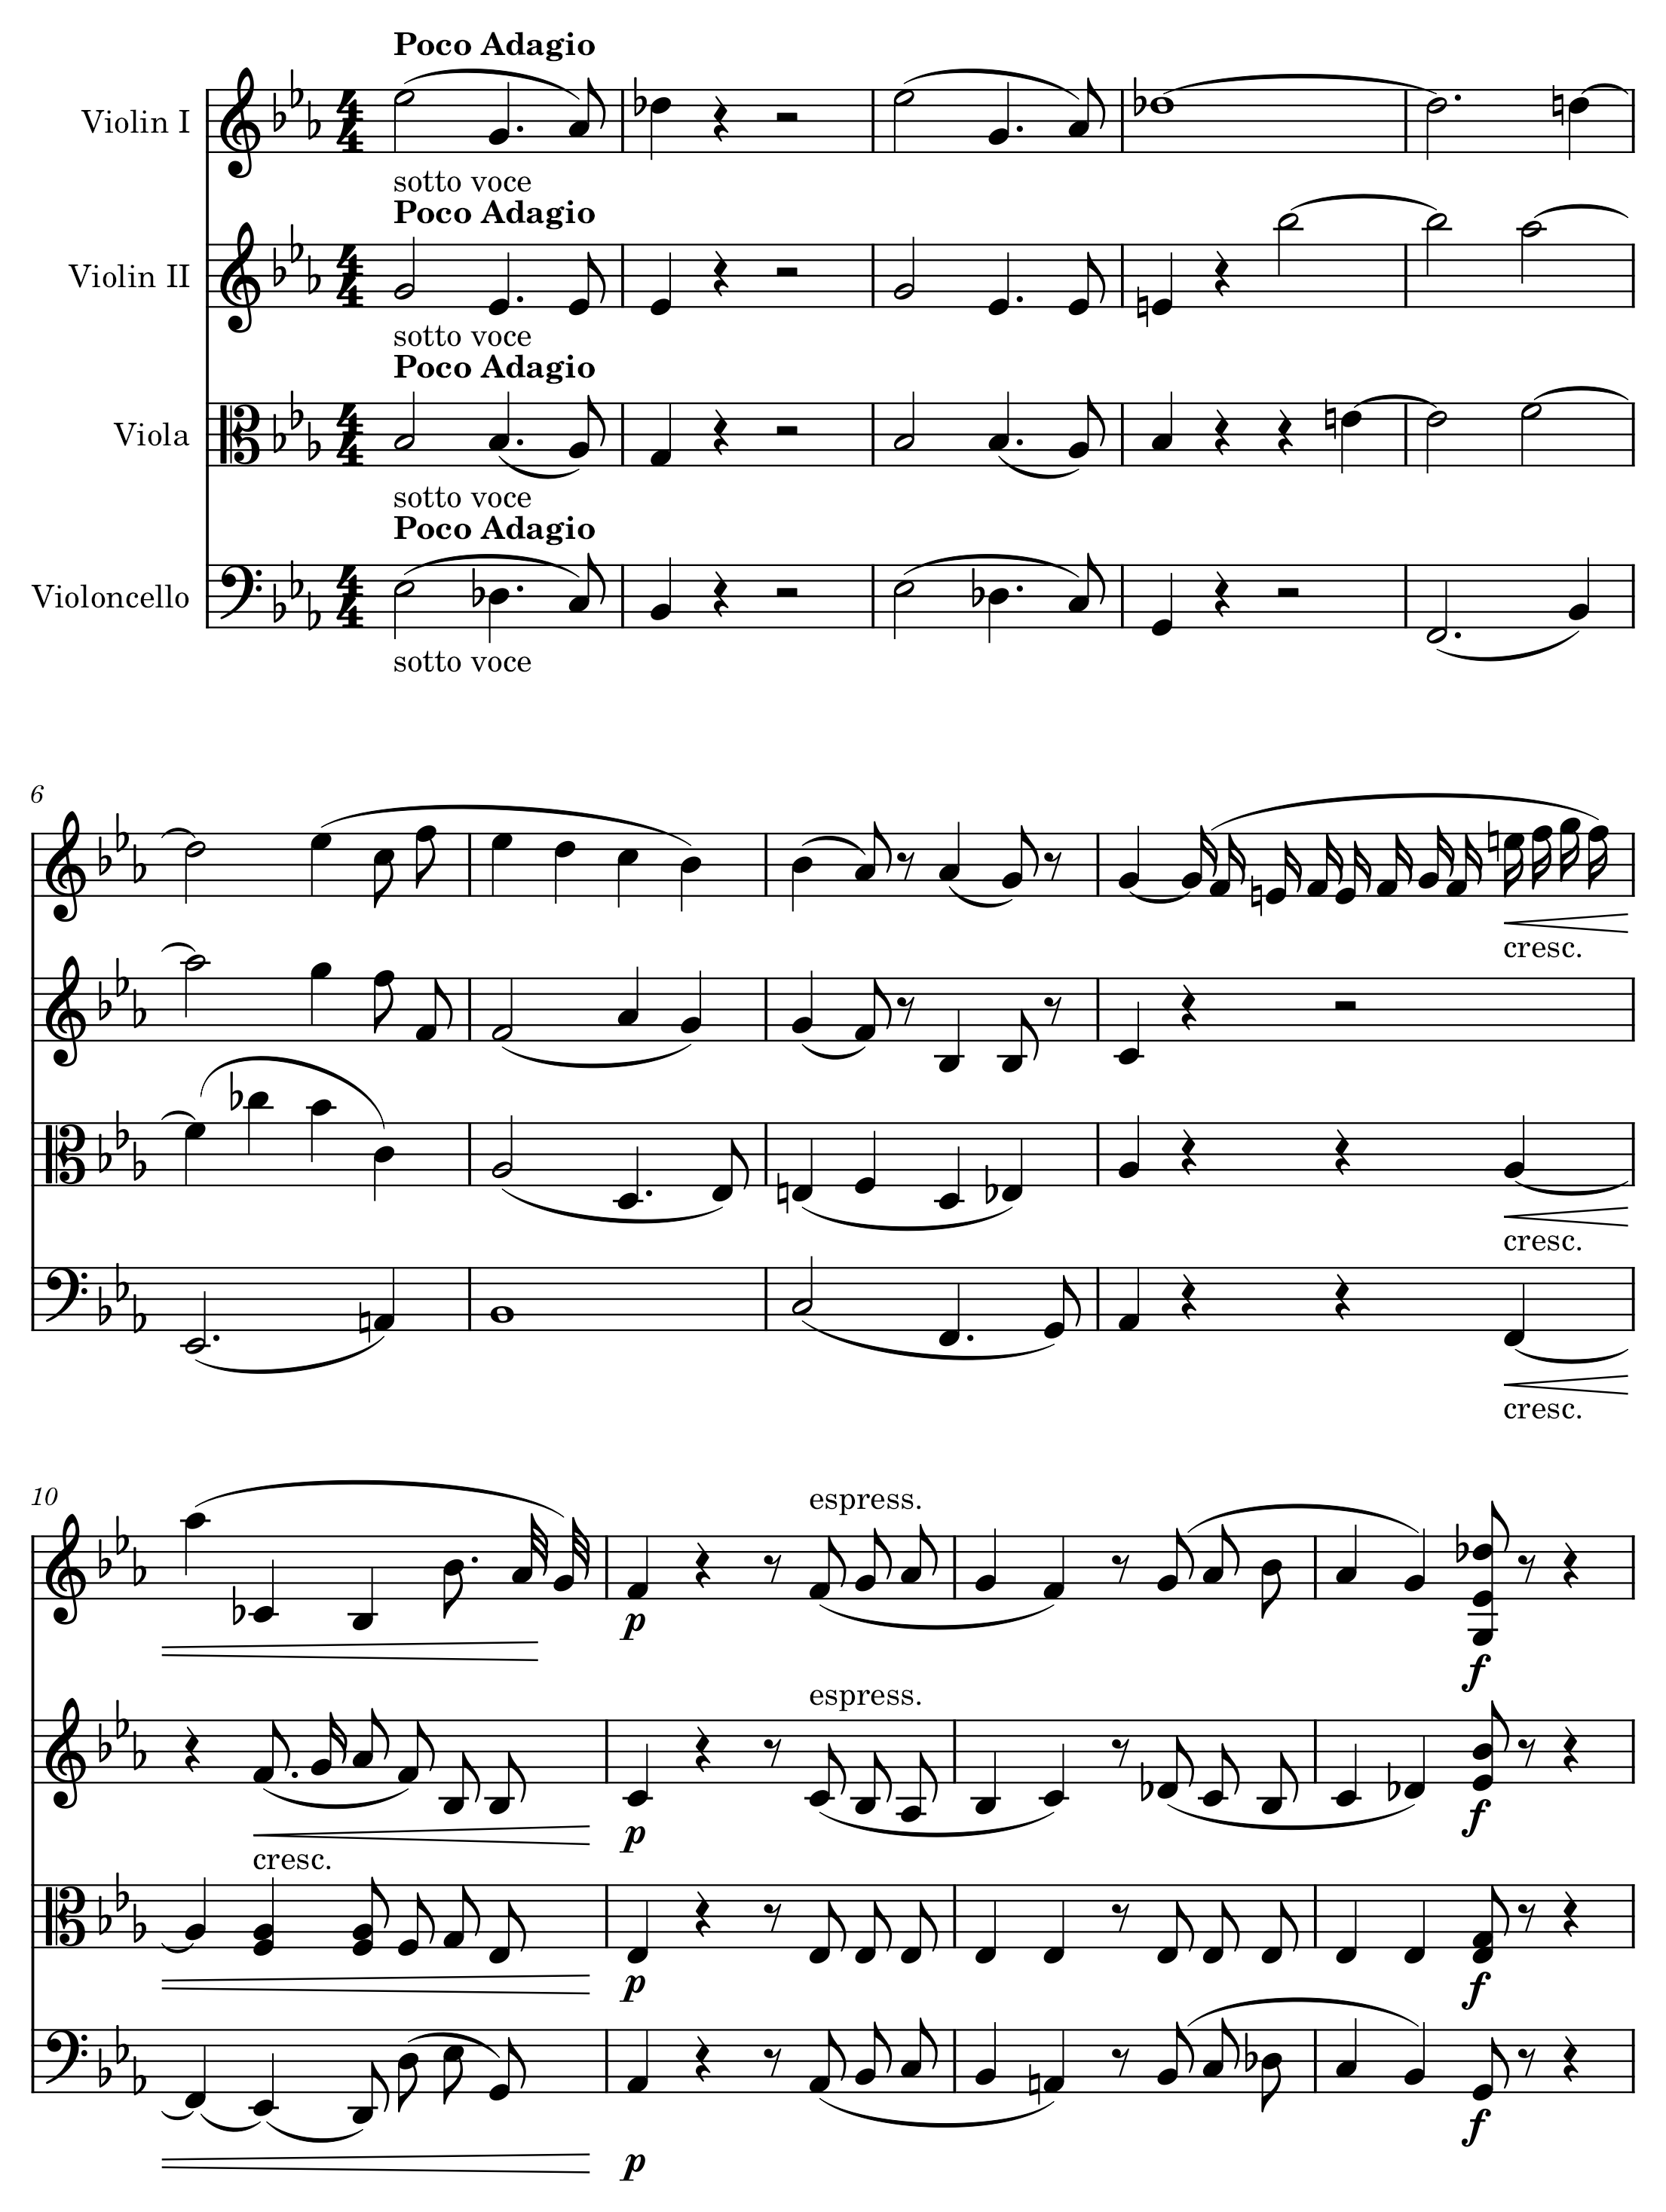
\includegraphics[width=0.5\textwidth]{../Figures/excerpt-1.png}
        \caption{String Quartet No.\ 10 by Ludwig van Beethoven}
    \end{figure}

    \note<1->{\begin{itemize}
        \item{Excerpt of String Quartet No. 10 in E-flat major, Op. 74, by Ludwig van Beethoven}
        \item{Chosen due to its relatively simple structure and smaller instrumentation, keeping the problem graph small}
    \end{itemize}}
\end{frame}

\begin{frame}{Phrase detection}
    \begin{figure}
        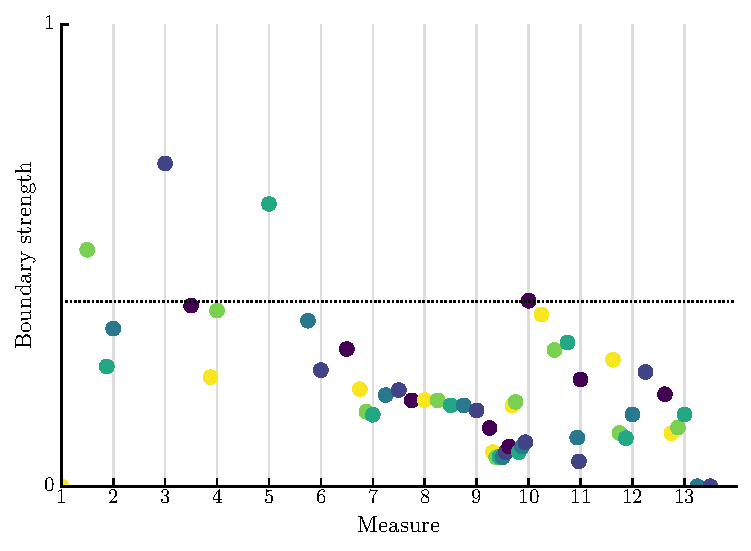
\includegraphics[width=0.75\textwidth]{../Figures/boundaryStrength_pad.pdf}
        \caption{Boundary strengths for the Violin I part}
    \end{figure}

    \note<1->{\begin{itemize}
        \item{Example of the LBDM finding suitable boundaries for phrases}
        \item{Threshold value of $0.4$ chosen, finds five phrases}
    \end{itemize}}
\end{frame}

\begin{frame}{Problem graph}
    \begin{figure}
        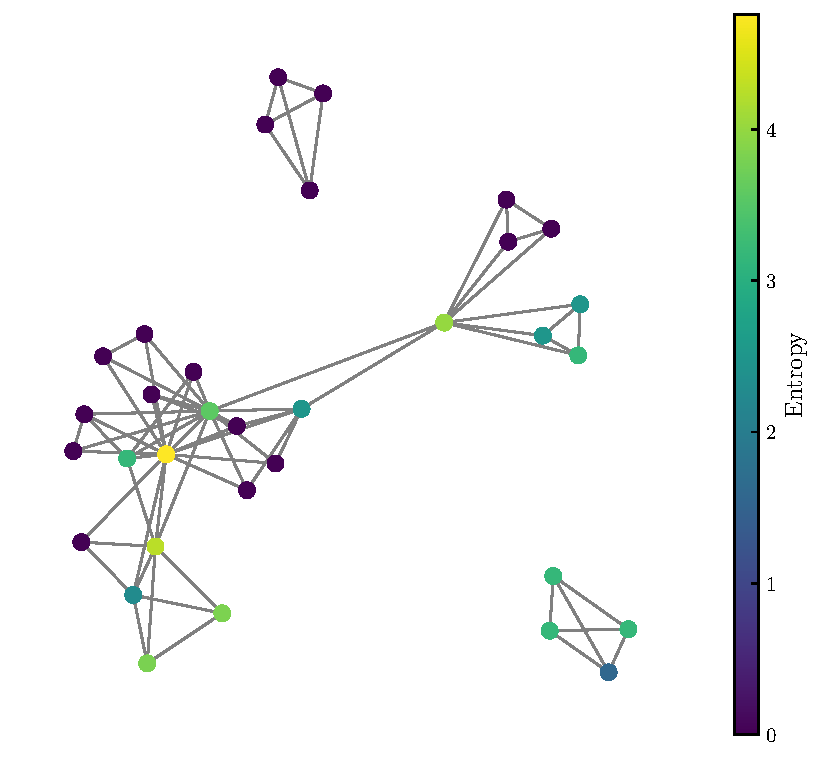
\includegraphics[width=.6\textwidth]{../Figures/problemGraph_pad.pdf}
        \caption{Problem graph with 33 nodes and 70 edges}
    \end{figure}

    \note<1->{\begin{itemize}
        \item{33 identified phrases (nodes) with 70 overlaps (edges)}
        \item{Nodes are weighted by the phrase entropy, how musically interesting the distribution of notes is}
    \end{itemize}}
\end{frame}

\begin{frame}{Solutions}
    \begin{figure}
        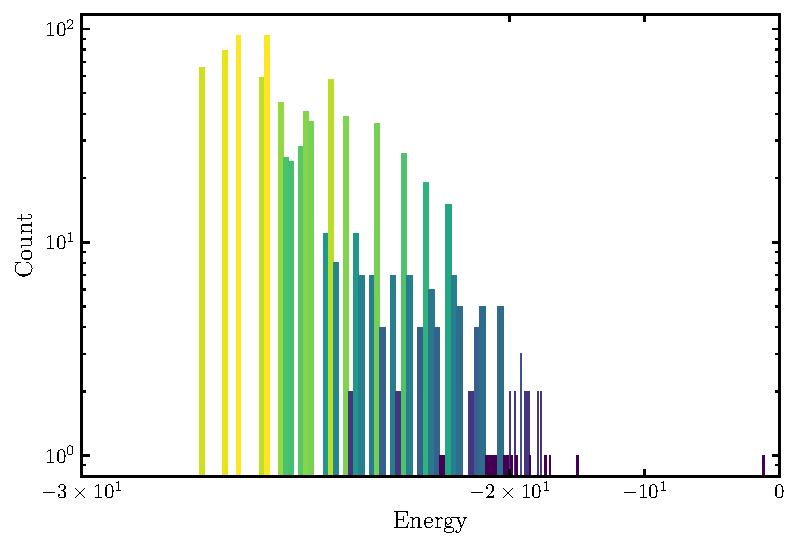
\includegraphics[width=0.8\textwidth]{../Figures/histogram_pad.pdf}
        \caption{Returned solutions for 1000 reads}
    \end{figure}

    \note<1->{\begin{itemize}
        \item{Histogram of the returned solutions, only energies below zero shown}
        \item{Distribution of solutions due to the stochastic nature of annealing}
        \item{Lowest energy solution most musically interesting due to construction of weighted MIS QUBO}
        \item{(Lowest energy solution $-26.8$ with a degeneracy of 34)}
    \end{itemize}}
\end{frame}

\begin{frame}{Example solution}
    \begin{figure}
        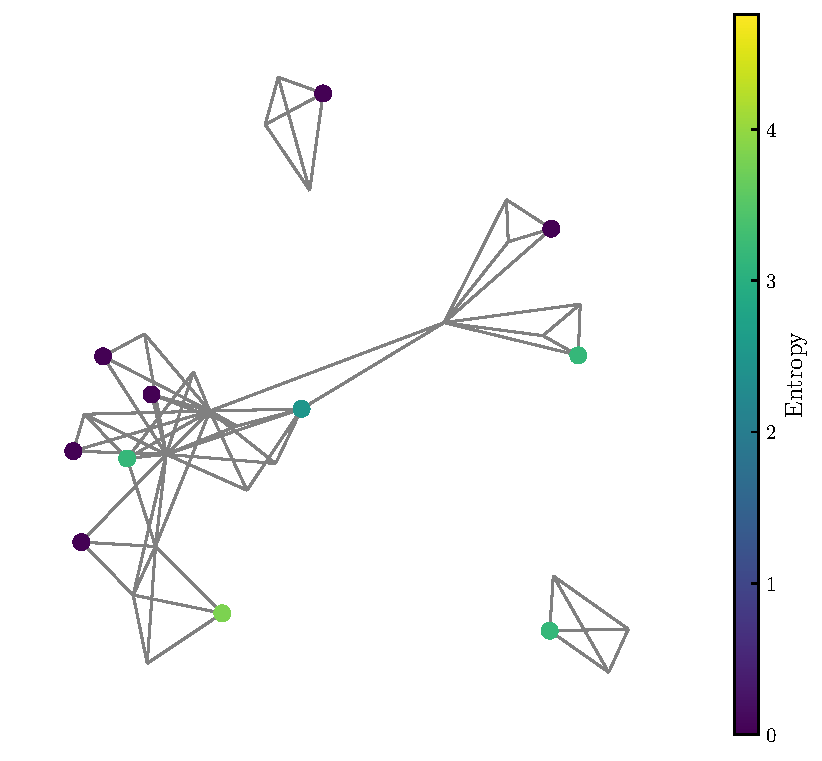
\includegraphics[width=.6\textwidth]{../Figures/solutionGraph_pad.pdf}
        \caption{Solution graph returning a subset of 11 nodes}
    \end{figure}

    \note<1->{\begin{itemize}
        \item{Selected nodes from one of the lowest energy solutions}
        \item{Note in the cliques only one node could be selected}
    \end{itemize}}
\end{frame}

\begin{frame}{Final arrangement}
    \begin{figure}
        \begin{subfigure}{0.5\linewidth}
            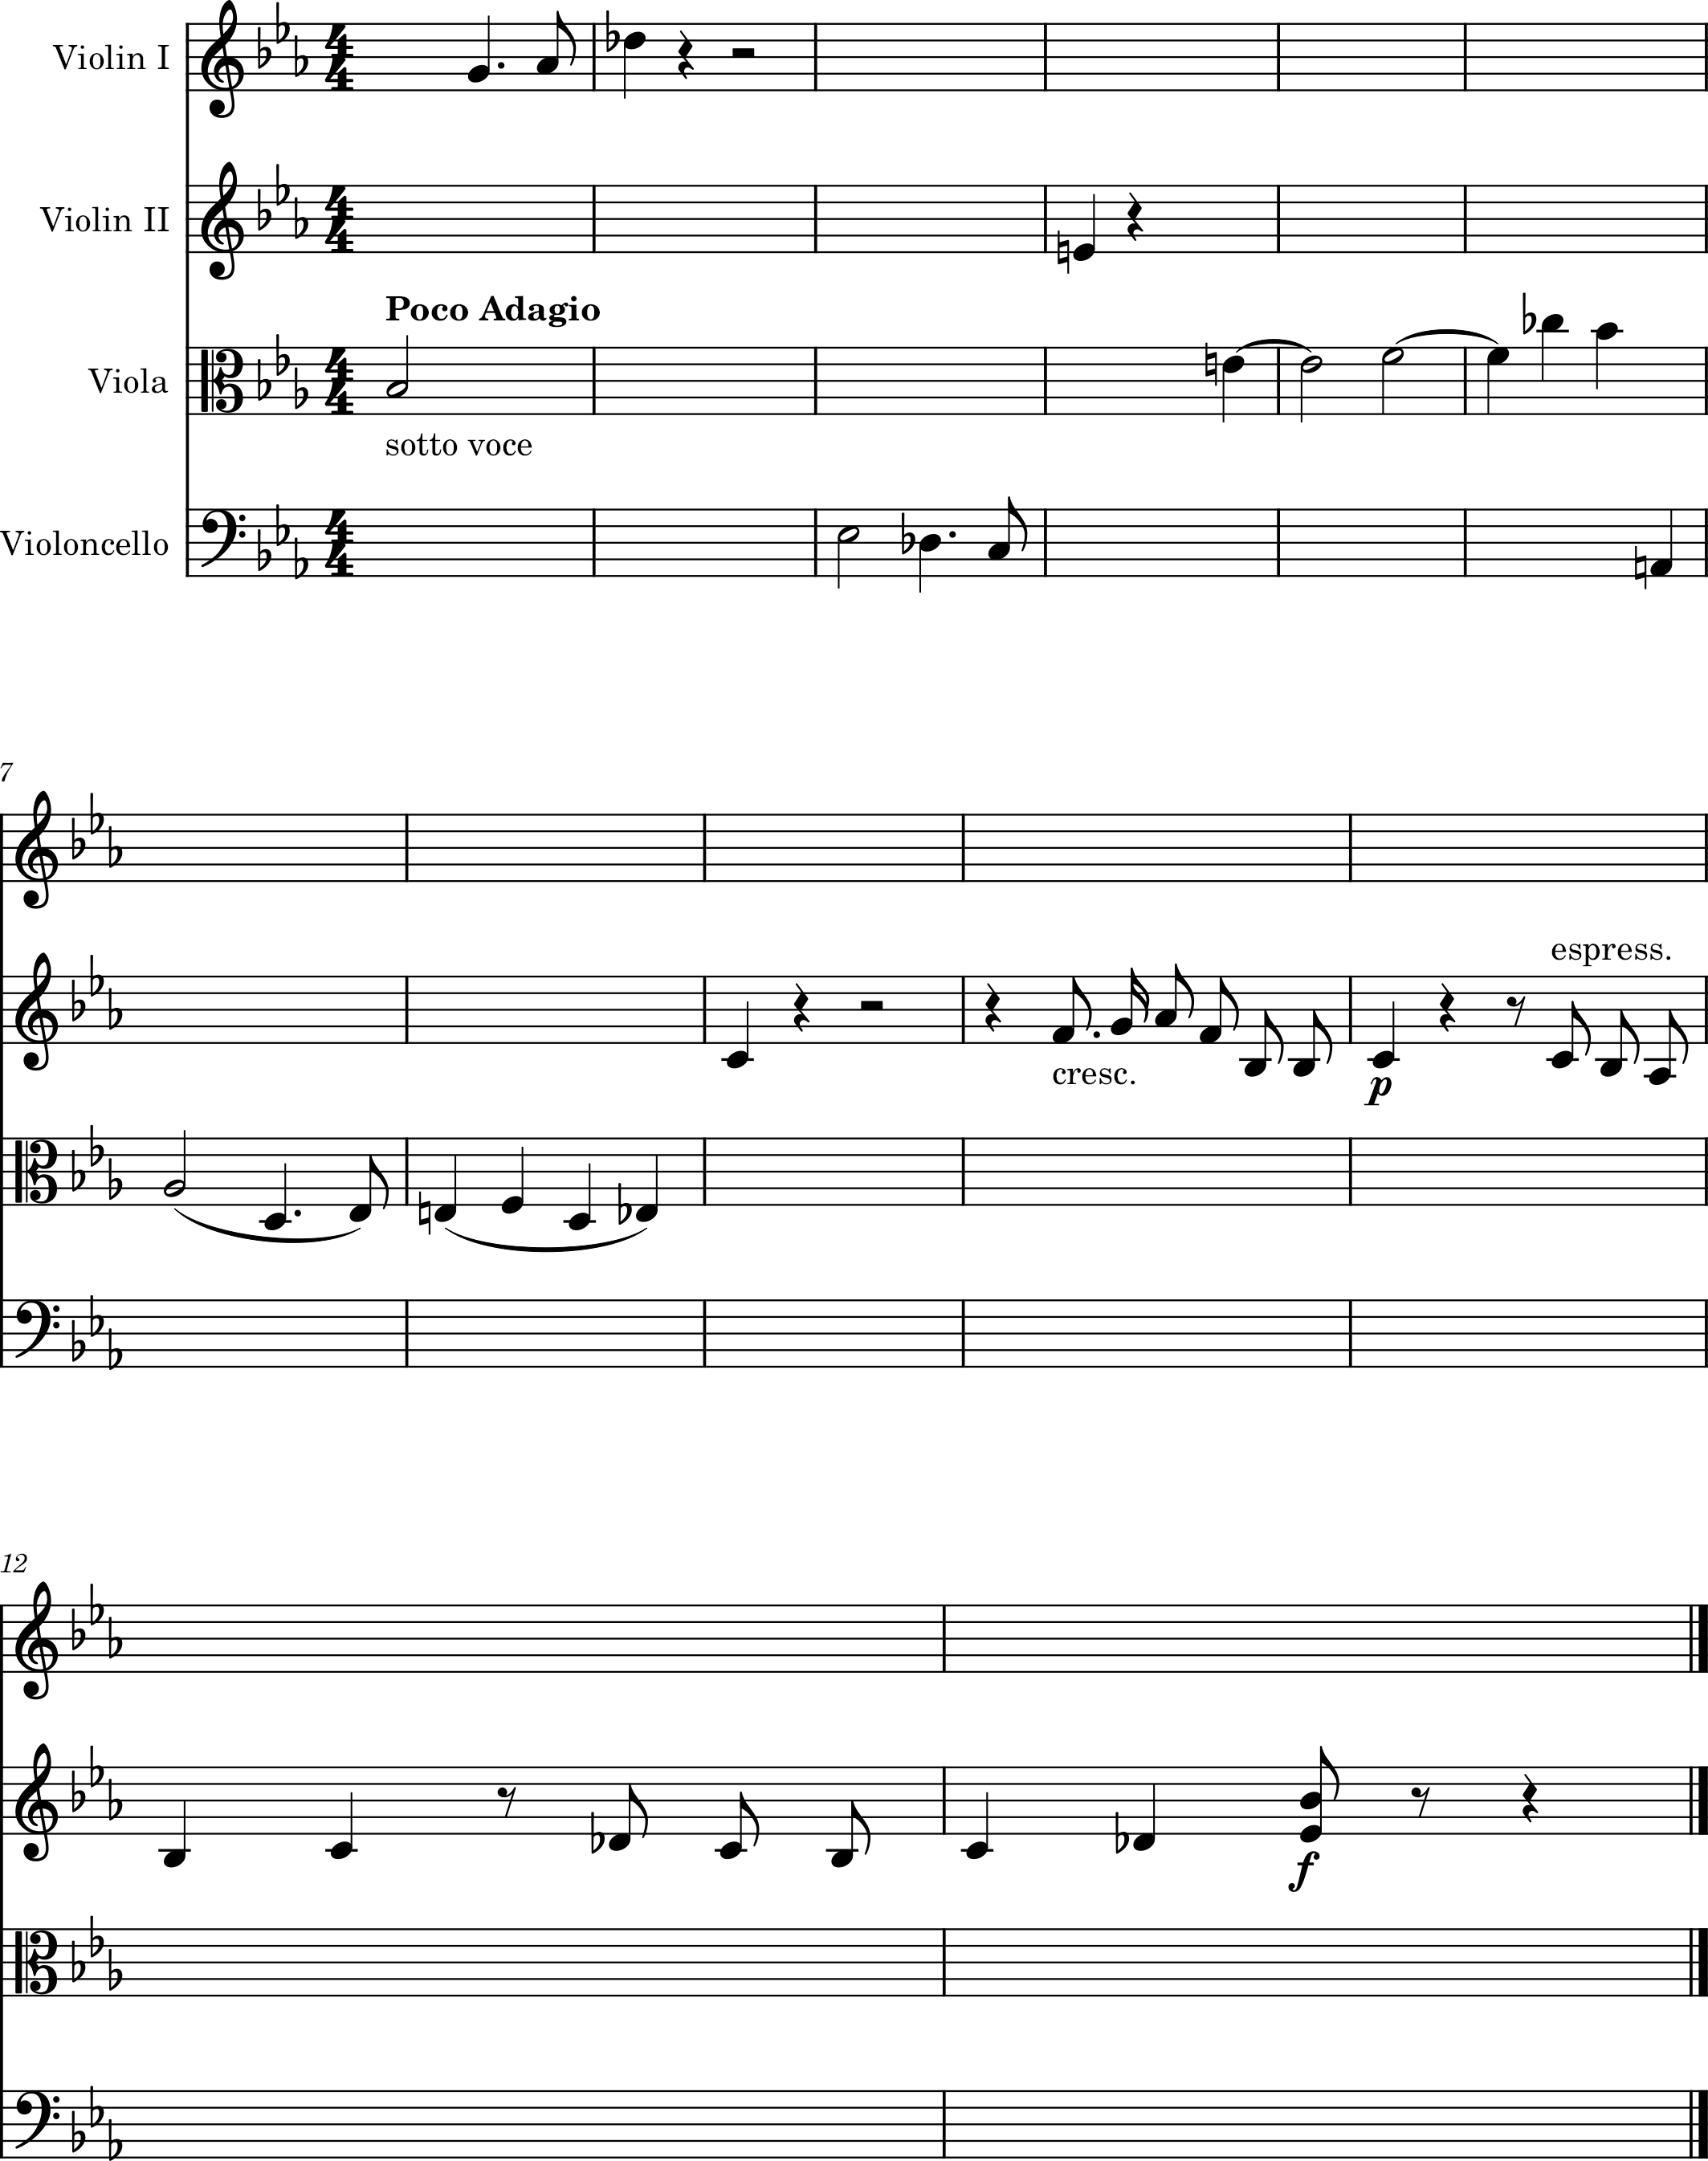
\includegraphics[width=.95\linewidth]{../Figures/selected-1.png}
            \caption{Selected phrases}
        \end{subfigure}\hfill
        \begin{subfigure}{0.5\linewidth}
            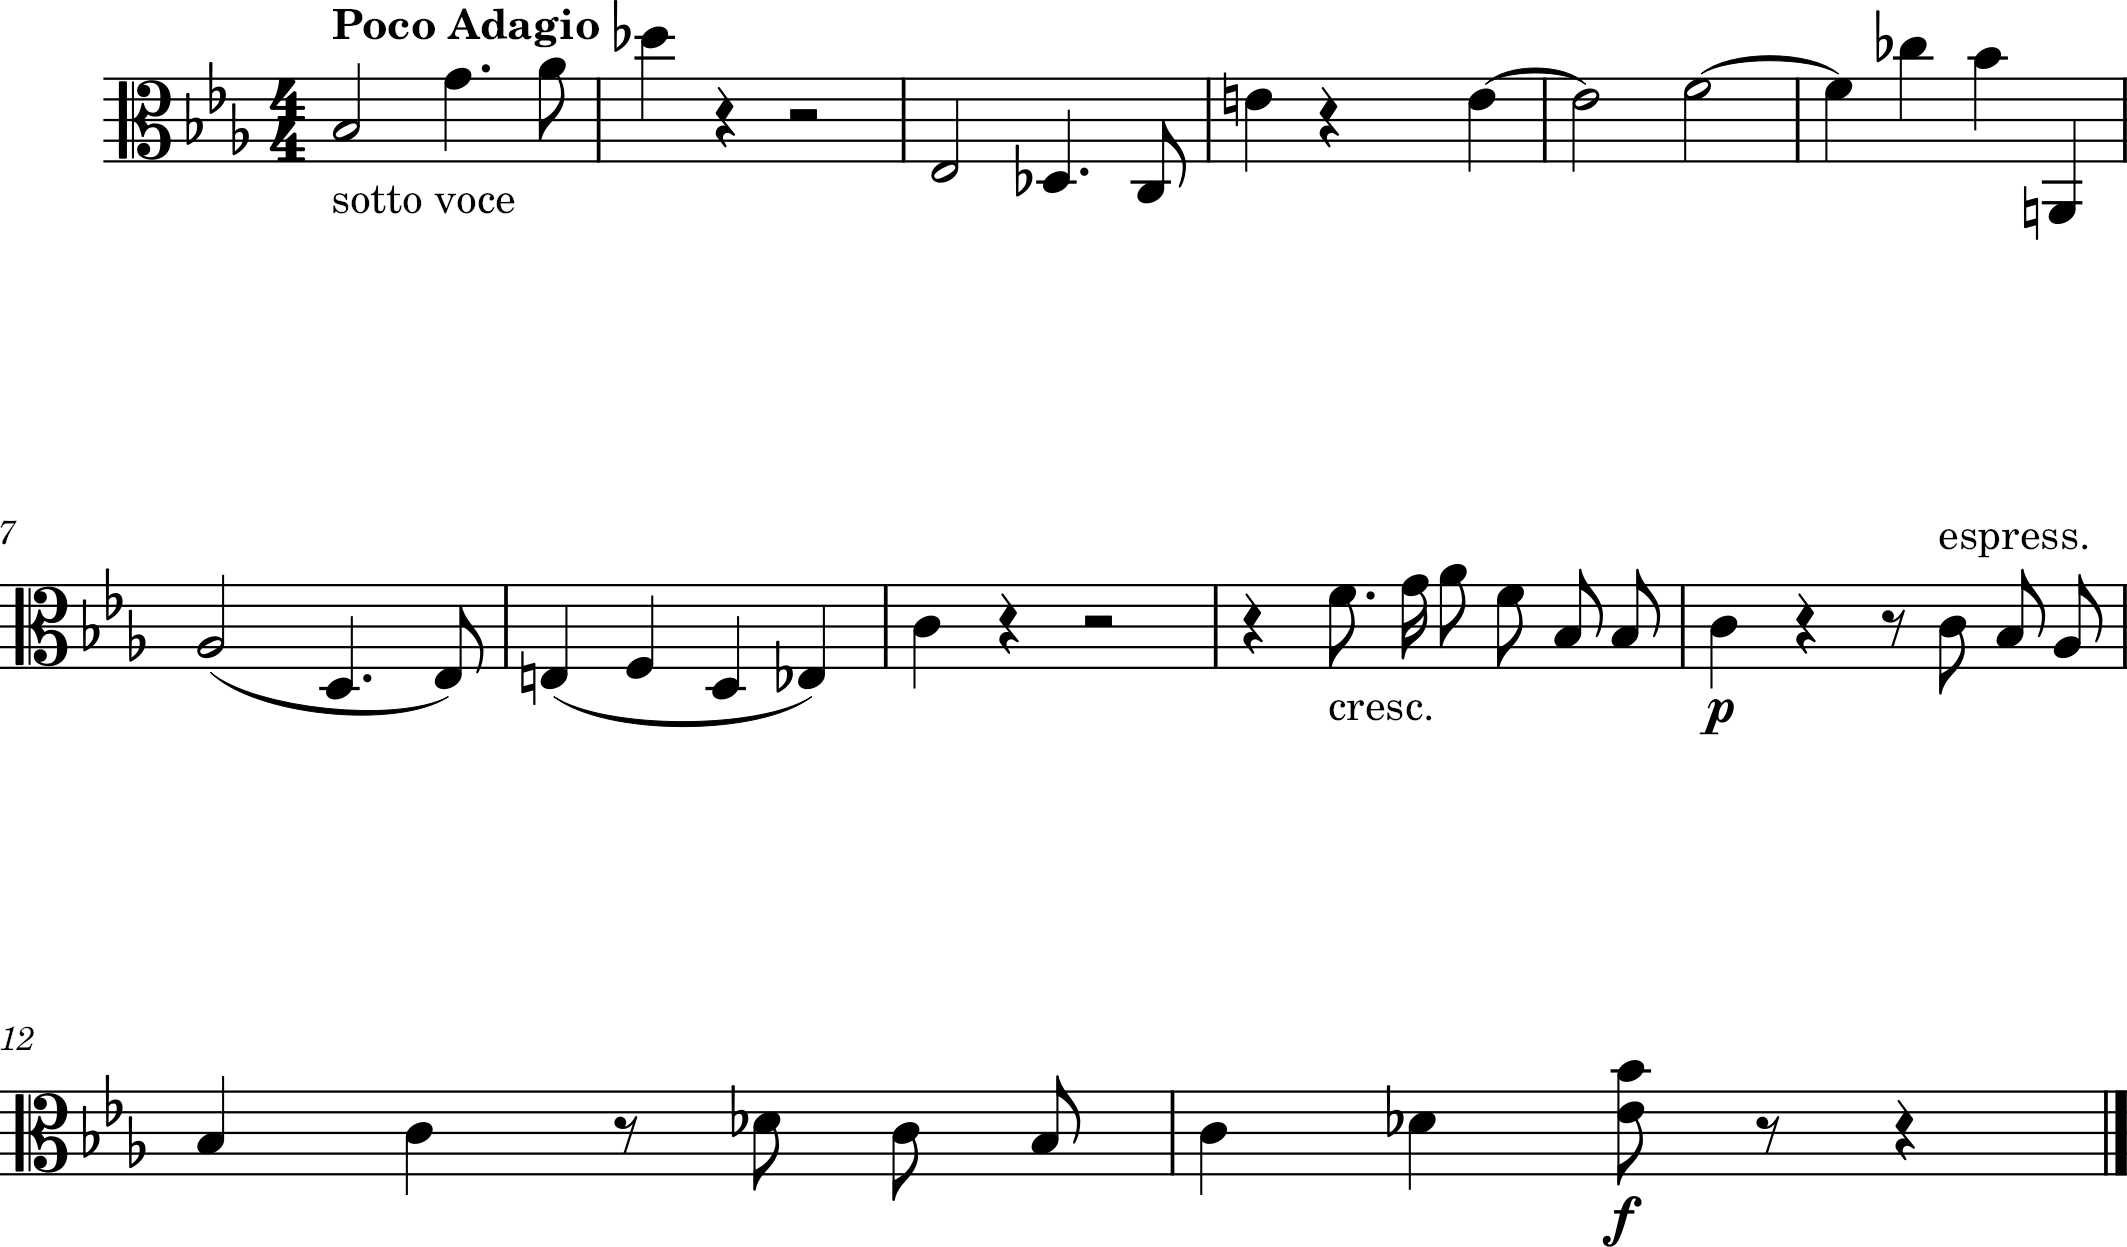
\includegraphics[width=.95\linewidth]{../Figures/arrangement-1.png}
            \caption{Final arrangement}
        \end{subfigure}
    \end{figure}

    \note<1->{\begin{itemize}
        \item{Selected phrases from solution graph highlighted}
        \item{Phrases concatenated to create the final arrangement}
    \end{itemize}}
\end{frame}

\section{Conclusions}

\begin{frame}{Conclusions}
    \begin{itemize}[<+(1)->]
        \item Successful in creating a valid single-part reduction
        \item Advantage over classical algorithms \cite{huang_towards_2012}
        \item Removes skill barrier for music arrangement
    \end{itemize}
    \begin{figure}
        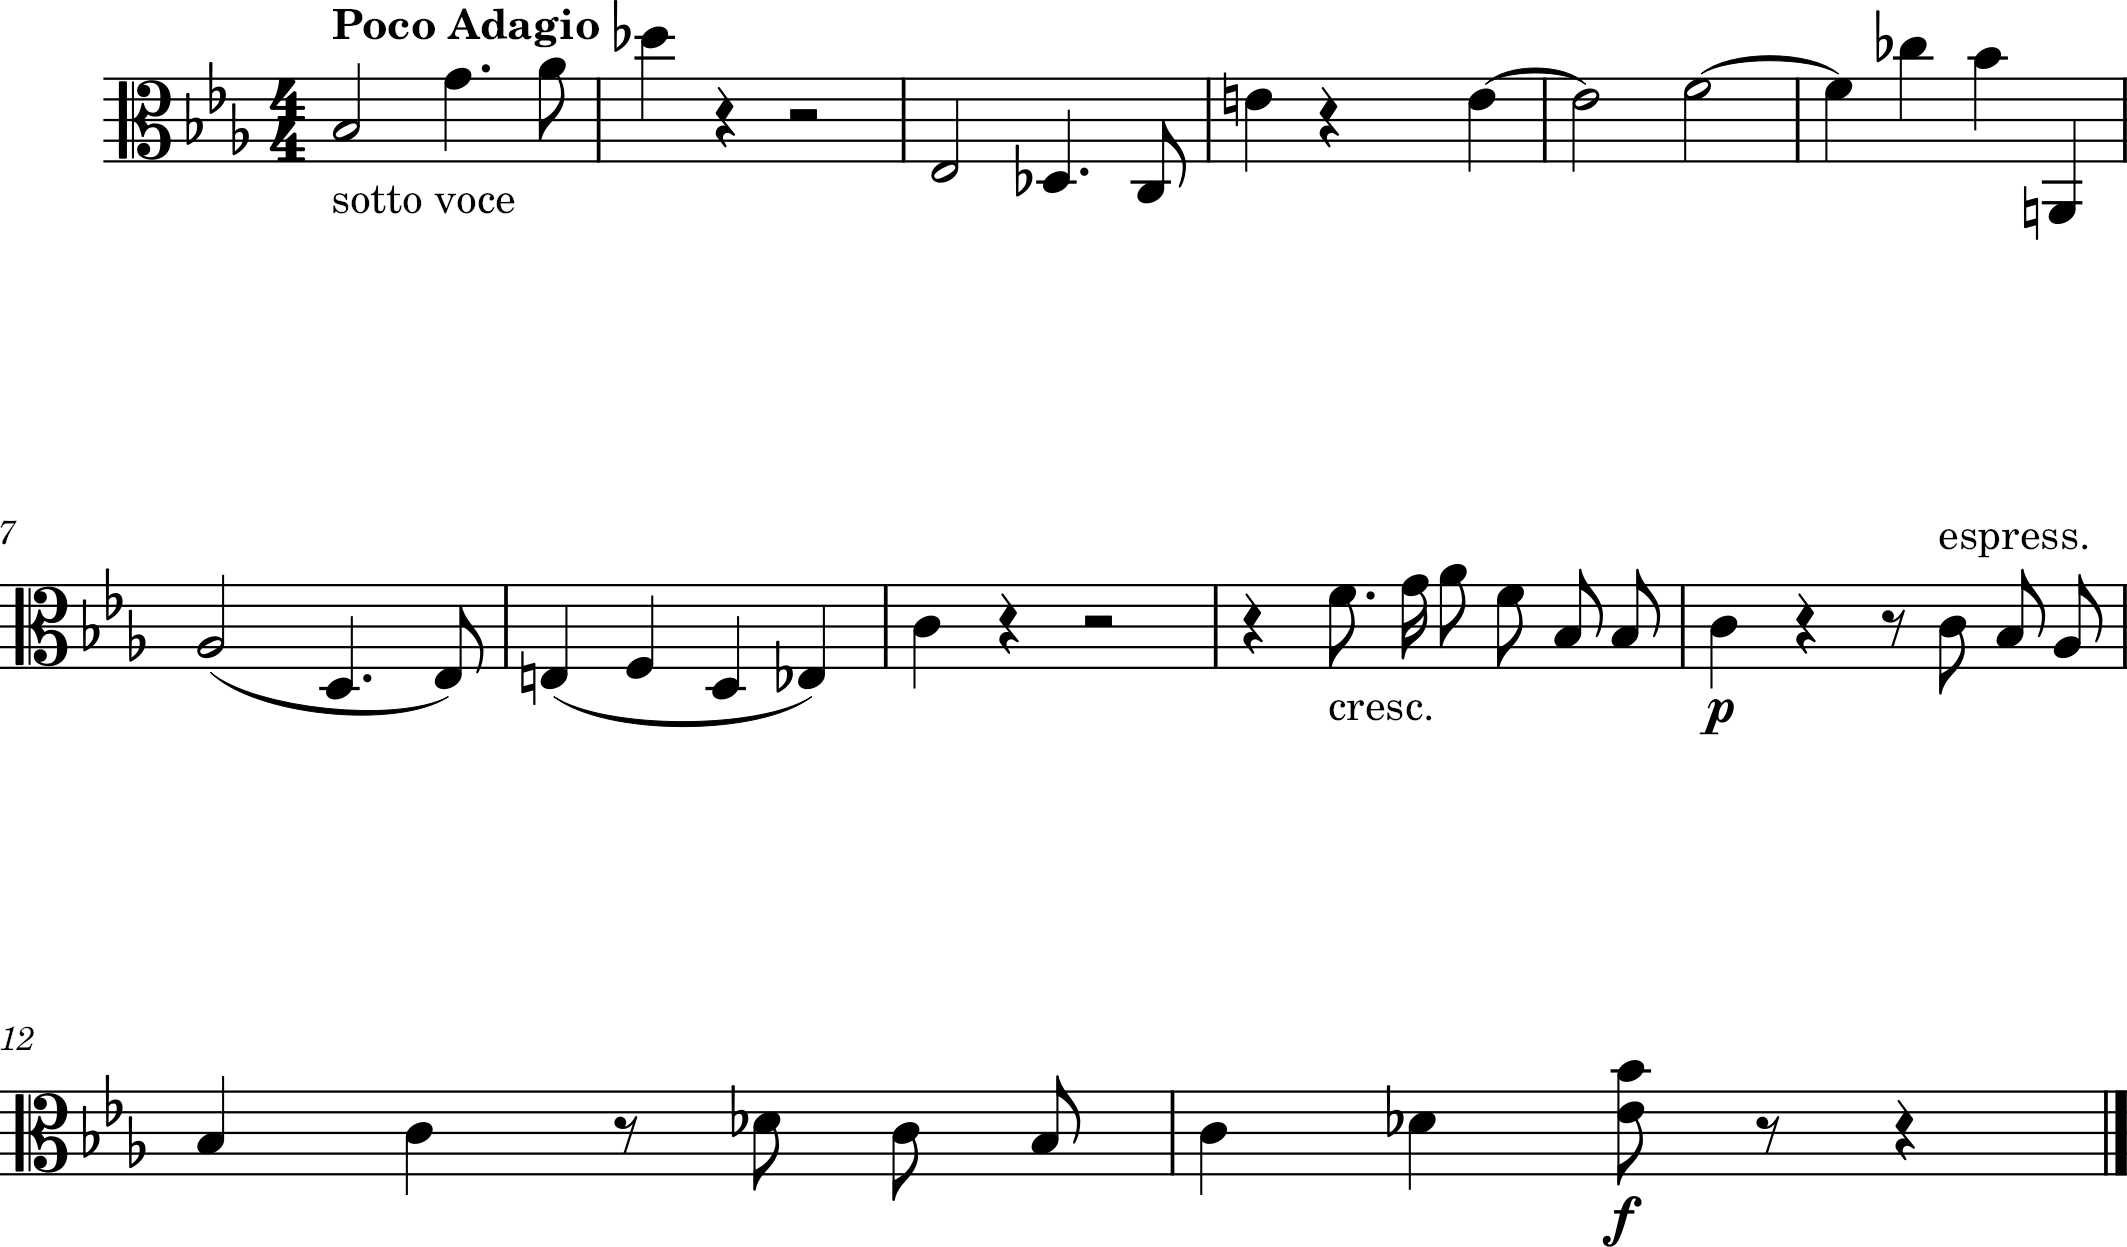
\includegraphics[width=.5\linewidth]{../Figures/arrangement-1.png}
    \end{figure}

    \note<1->{\begin{itemize}
        \item{Valid reduction gained from implemented method}
        \item{Monophonic lowest-energy solution}
        \item{Phrase identification and selection result in musically interesting final arrangement}
        \item{Displays some advantages over classical algorithms}
        \item{Does not require training data, costly in both time and resources}
        \item{Faster solve time compared to similarly-sized problems}
        \item{Method and more advanced versions of it removes the skill barrier for music arrangement}
    \end{itemize}}
\end{frame}

\begin{frame}{Future work}
    \begin{itemize}[<+(1)->]
        \item Increased problem size
        \item Parametric variation of LBDM
        \item Physical limitations of instruments
        \item Reduction to more than one part
        \item Quality comparison of computer arrangements \cite{pearce_towards_2001}
    \end{itemize}

    \note<1->{\begin{itemize}
        \item{Problem size | full piece has upwards of 1000 phrases, compare solve times with classical algorithms}
        \item{LBDM parameters | phrases should be short and similar in length, prevents important notes being hidden in long phrases with low entropy}
        \item{Physical limitations | note ranges, note change speed}
        \item{Multiple parts | need different problem formulation, colouring problem with each colour representing a reduced part}
        \item{Quality judgement | Turing-like test, present subjects with human-/computer-generated scores}
    \end{itemize}}
\end{frame}

\begin{frame}[standout]
    Thank you!
\end{frame}

\appendix

\begin{frame}
    \titlepage
\end{frame}

\begin{frame}{LBDM}
    \begin{block}{Boundary strength}
        \begin{gather*}
            S_i=x_i\times (r_{i-1, i} + r_{i, i+1}) \\
            r_{i, i+1}=\frac{|x_{i}-x_{i+1}|}{x_{i}+x_{i+1}}
        \end{gather*}
    \end{block}
    \begin{block}{Normalisation}
        \begin{equation*}
            S_i'=\frac{S_i-\min(S_i)}{\max(S_i)-\min(S_i)}
        \end{equation*}
    \end{block}
    \begin{block}{Weighting}
        \begin{equation*}
            S=\frac{1}{3}\left( S'_\mathrm{pitch} + 2 S'_\mathrm{IOI} \right)
        \end{equation*}
    \end{block}
    \hfill\cite{cambouropoulos_lbdm_2011}

    \note{\begin{itemize}
        \item{Boundaries always taken at beginning/end of piece}
        \item{Weightings derived by trial and error}
    \end{itemize}}
\end{frame}

\begin{frame}{MIS}

    \begin{equation*}
        f(x)=A\sum_{ij\in E}x_ix_j-B\sum_i W_ix_i
    \end{equation*}
    \hfill\cite{lucas_ising_2014}

    $A/B>=2\max(W)$ to weight the constraint term more heavily than any objective term

    \note{\begin{itemize}
        \item{Weighted MIS QUBO}
        \item{Lagrange paramters $A$/$B$ determine the balance between constraint and objective}
    \end{itemize}}
\end{frame}

\begin{frame}{Phrase entropy}
    \begin{block}{Shannon entropy}
        \begin{equation*}
            H(X)\coloneq-\sum_i P(x_i)\log_2 P(x_i)
        \end{equation*}
    \end{block}
    \begin{block}{Probability distribution}
        \begin{equation*}
            P(x_i)=\frac{n_i}{N}
        \end{equation*}
    \end{block}
    \hfill\cite{li_automatic_2019}

    \note{\begin{itemize}
        \item{Shannon entropy units in bits due to $\log_2$}
        \item{Distribution calculated for pitch and duration}
    \end{itemize}}
\end{frame}

\end{document}